\RequirePackage{fix-cm}
\documentclass{article}
\usepackage{graphicx}
\usepackage{background}
\usepackage{tikz}
\usepackage{float}
\usepackage{eso-pic}
\usepackage{hyperref}


% Imposta il background per la prima pagina
\backgroundsetup{
    scale=1,
    color=black,
    opacity=1,
    angle=0,
    contents={
        \begin{tikzpicture}[overlay, remember picture]
            \node[inner sep=0pt, anchor=center] at (current page.center) {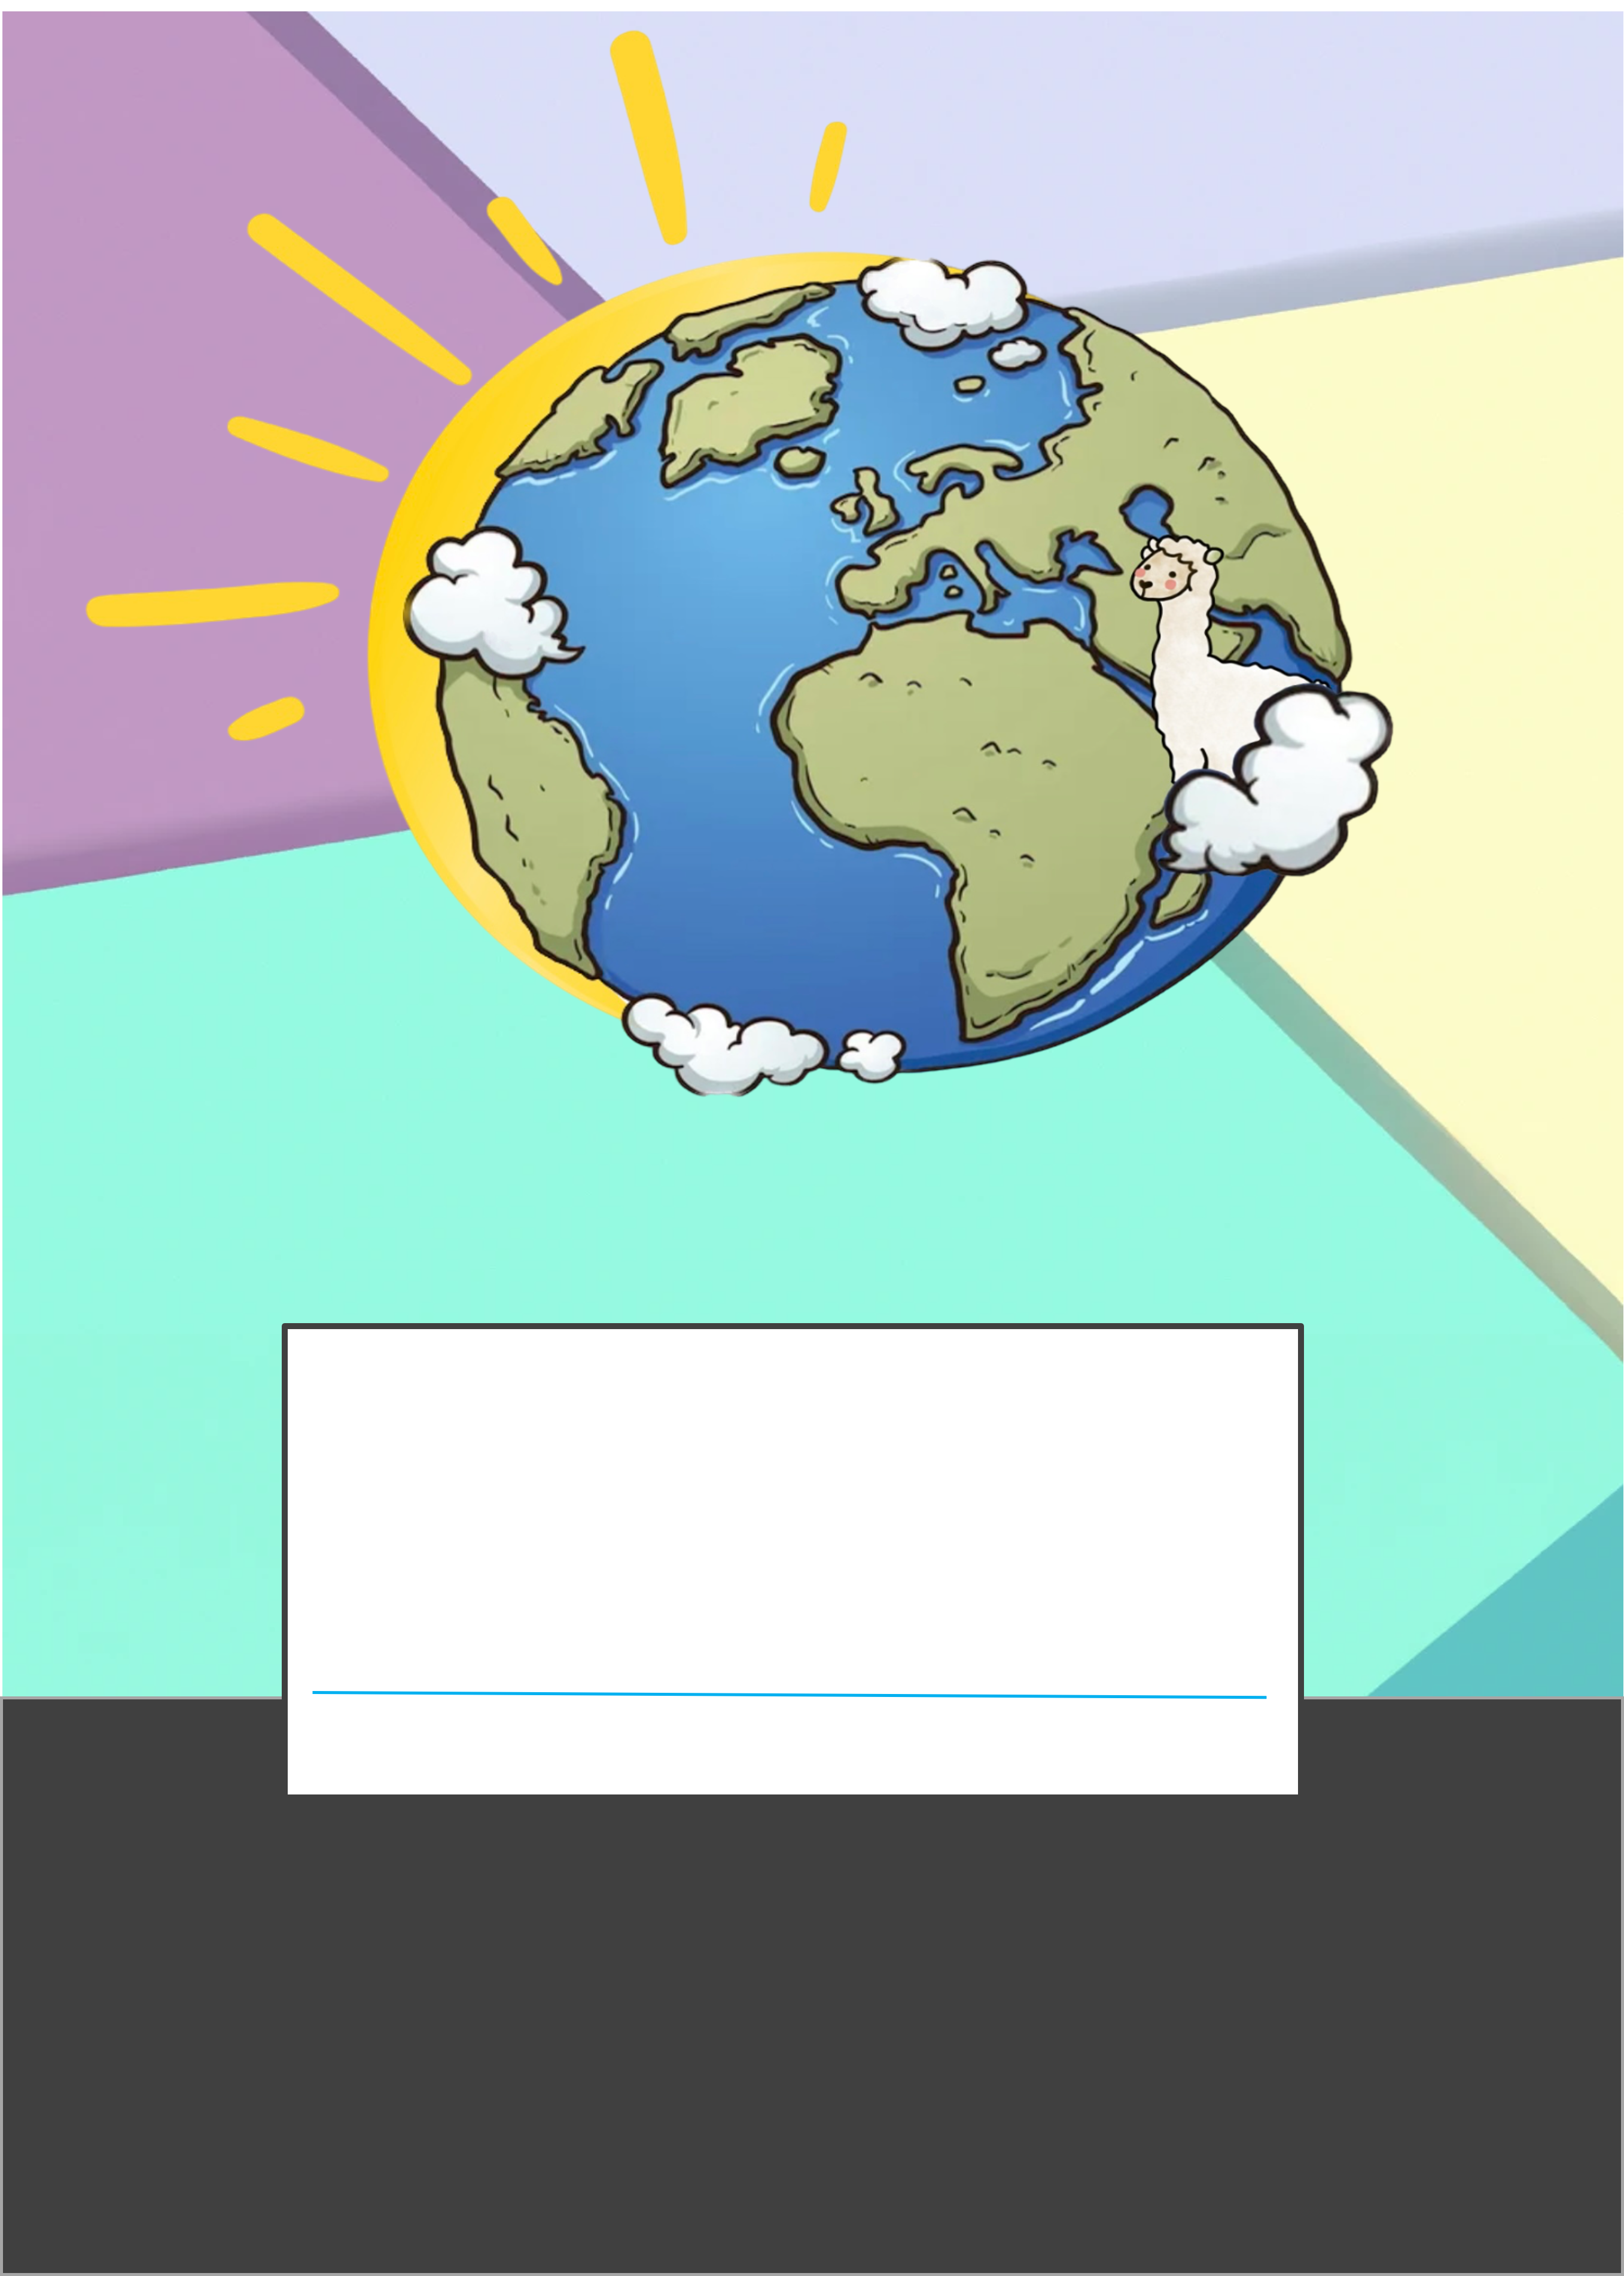
\includegraphics[width=\paperwidth,height=\paperheight,keepaspectratio]{../../img/firstpage_background.png}};
            \node[text=cyan, font=\fontsize{35}{50}\selectfont\bfseries] at ([xshift=-0.2cm,yshift=-4.5cm]current page.center) {Climate Monitoring};
            \node[text=cyan, font=\large] at ([xshift=-0.4cm,yshift=-7.5cm]current page.center) {\textit{Manuale Tecnico}};
            \node[text=white, font=\large] at ([xshift=-8.5cm,yshift=-9cm]current page.center) {Autori:};
            \node[text=white, font=\large] at ([xshift=-6.85cm,yshift=-10.5cm]current page.center) {Andrea Tettamanti 745387};
            \node[text=white, font=\large] at ([xshift=-7.28cm,yshift=-11.5cm]current page.center) {Luca Mascetti 752951};
            \node[text=white, font=\large] at ([xshift = 8cm, yshift = -9cm]current page.center) {Versione: 1.1};
            \node[text=white, font=\large] at ([xshift = 8cm, yshift = -10cm]current page.center) {Data: 07-02-2024};
        \end{tikzpicture}    }
}



\begin{document}



%frontespizio
\begin{titlepage}
    \null
\end{titlepage}

% Sovrapponi l'immagine al numero di pagina
\AddToShipoutPictureBG{
    \begin{tikzpicture}[overlay, remember picture]
        \node[inner sep=0pt, anchor=south] at ([xshift=-0.15cm,yshift=2.7cm]current page.south) {
\includegraphics[width=1.5cm,height=1.5cm]{../../img/number page.png}};
    \end{tikzpicture}
}

\clearpage
\NoBgThispage
\tableofcontents
\listoffigures
\clearpage


\NoBgThispage
\section{Introduzione}
Benvenuti nell'applicazione \emph{Climate Monitoring}, software progettato per fornire accesso ai dati climatici 
provenienti dai centri di monitoraggio in tutta Italia. Questa applicazione è stata sviluppata con l'obiettivo di 
mettere a disposizione degli operatori ambientali e dei cittadini comuni dati accurati e rilevanti relativi alle 
condizioni climatiche della propria zona di interesse.

\section{Progettazione}

Il software è stato progettato seguendo un approccio client-server, in cui il server si occupa di ricevere i dati dai client e memorizzarli nel database, mentre i client possono richiedere i dati memorizzati al server.\\
Per la parte client, viene seguita l'architettura CMV (Controller-Model-View), in cui il controller e il view sono uniti nelle classi dell'interfaccia grafica, mentre il model è separato in un package a parte che 
permette l'uso dei metodi degli oggetti remoti presenti nel server. Questo viene fatto attraverso l'uso della tecnologia java RMI (Remote Method Invocation).
\NoBgThispage
\section{Struttura Generale dell'Applicazione}
L’applicazione è stata sviluppata seguendo l’architettura \texttt{MVC (Model-View-Controller)}, dove le parti View e Controller sono inglobati nella User Interface (UI).
Di conseguenza il codice sorgente del package \texttt{src} è suddiviso in due Macro-package: \texttt{Models} in cui sono presenti tutte le classi che gestiscono i dati,
mentre nel package \texttt{GUI} sono presenti le classi che gestiscono la UI e l’interazione tra i comandi fatti dall’utente e lo storage dei dati.
È presente anche un package, \texttt{utils}, che contiene classi di utilità usate nella maggior parte delle altre classi.


\begin{figure}[H]
    \centering
    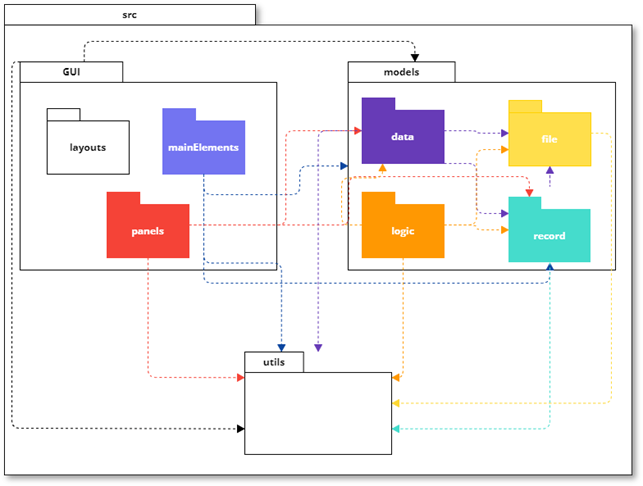
\includegraphics[width=0.7\textwidth]{../../img/package_structure.png}
    \caption{Struttura dei package dell'applicazione.}
\end{figure}
\section{Package Server}
In questa sezione verranno descritti il package \texttt{server} e le classi che lo compongono.\\

\begin{figure}[H]
    \centering
    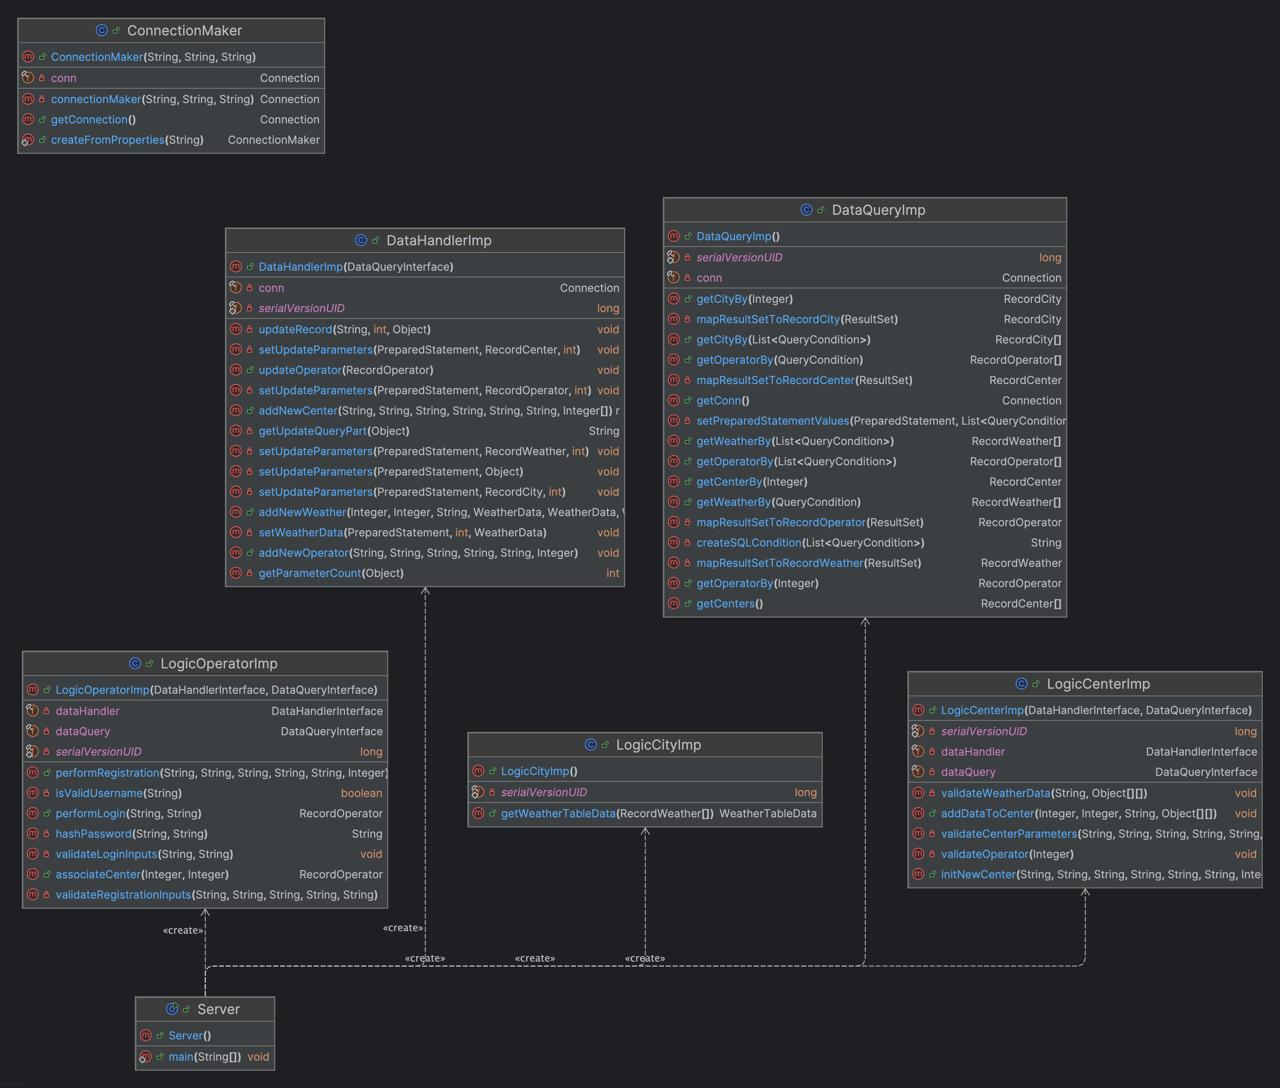
\includegraphics[width=0.9\textwidth]{img/serverClassDiagram.jpg}
    \caption{UML del package Server}
    \label{fig:Server}
\end{figure}

\subsection{Server}
La classe \texttt{Server} è progettata per avviare il registro RMI e pubblicare le implementazioni delle interfacce remote.\\
Queste implementazioni sono accessibili ai client remoti, che possoo invocare metodi per interrogare, gestire e manipolare i dati relativi alle operazioni dell'applicazione.\\
In sisntesi, \texttt{Server} svolge le seguenti operazioni principali:
\begin{itemize}
    \item \textbf{Creazione e Configurazione del Registro RMI}: avvia un registro RMI sulla porta specificata (di default, la porta 1099) utilizzando il metodo\\
          \texttt{LocateRegistry.createRegistry(int port)}. Questo registro permette ai client remoti di trovare e invocare i metodi delle interfacce registrate.
    \item \textbf{Inizializzazione delle Implementazioni RMI}: la classe crea istanze delle implementazioni delle interfacce remote che gestiscono diverse logiche di business.
          Queste implementazioni sono
          \begin{itemize}
              \item \texttt{DataQueryImp}
              \item \texttt{DataHandlerImp}
              \item \texttt{LogicOperatorImp}
              \item \texttt{LogicCenterImp}
              \item \texttt{LogicCityImp}
          \end{itemize}
    \item \textbf{Registrazione delle Implementazioni nel Registro RMI}: ogni implementazione viene registrata nel registro RMI con un nome specifico utilizzando il metodo
          \texttt{rebind(String name, Remote obj)}. Questo passaggio rende i metodi delle interfacce remote accessibili ai client remoti trmite il nome associato.
\end{itemize}

\subsection{ConnectionMaker}
La classe \texttt{ConnectionMaker} è progettata per gestire la connessione al database, utilizzando sia parametr5i espliciti che file di configurazione.\\
La gestione della connessione viene effettuata tramite l'oggetto \texttt{Connection}, che rappresenta un collegamento la database, permettendo l'esecuzione di query e altre operazioni di manipolazione dei dati.\\
\\
I metodi pubblici sono:
\begin{itemize}
    \item \texttt{createFromProperties(String filepath)}:
          questo metodo statico consente di creare un'istanza di \texttt{ConnectionMaker} utilizzando un file di properties. Il file specificato deve contenere le chiavi \texttt{db.url}, \texttt{db.username} e \texttt{db.password},
          che vengono lette e utilizzate per stabilire la connessione al databse.
          Se il file non viene trovato o si verifica un errore durante la lettura, viene lanciata un'eccezione.
    \item \texttt{getConnection()}:
          questo metodo pubblico restituisce l'oggetto \texttt{Connection} gestito da \texttt{ConnectionMaker}. Questo permette ad altre classi del sistema di accedere alla connessione per eseguire operazioni di query, aggiornamento o altre interazioni con il database.
\end{itemize}
I metodi privati sono:
\begin{itemize}
    \item \texttt{connectionMaker(String url, String username, String password)}:
          questo metodo privato è responsabile della creazione effettiva della connessione al databse. Utilizza l'URL, il nome utene e la password per creare un oggetto \texttt{Connection} tramite il \texttt{DriverManager} di JDBC. Il metodo configura anche un oggetto \texttt{Properties} pre gestire le credenziali di accesso.
\end{itemize}




\subsection{Package ImplementationRMI}
Il package \texttt{ImplementationRMI} contiene le classi che implementano le interfacce remote definite nel package \texttt{InterfacesRMI} e che gestiscono le logiche di business dell'applicazione.\\


\subsubsection{DataHandlerImp}
La classe \texttt{DataHandlerImp} implementa l'interfaccia \texttt{DataHandlerInterface} e si occupa di gestire operazioni aggiunte e aggiornamento dei record nel database.
Questa classe utilizza JDBC per interagire con il database e fornisce metodi per gestire i record relativi agli operatori, ai centri di monitoraggio e ai dati climatici.\\
\\
I metodi pubblici sono:
\begin{itemize}
    \item \texttt{addNewOperator(String nameSurname, String taxcode, String email, String username, String password, Integer centerID)}:
          aggiunge un nuovo operatore al databse. Prima di inserire i dati, viene effettuato un controllo per assicurarsi che l'utente non esista già.
          Lancia eccezioni \texttt{SQLException, RemoteException, IllegalArgumentException} in caso di errori.
    \item \texttt{addNewCenter(String centerName, String streetName, String streetNumber, String CAP, String townName, String districName, Integer[] cityIDs)}:
          aggiunge un nuovo centro di monitoraggio al database. Prima di inserire i dati, viene effettuato un controllo per evitare duplicati. Restituisce un oggetto \texttt{RecordCenter} che rappresenta il centro appena inserito.
          Lancia eccezioni \texttt{SQLException, RemoteException, IllegalArgumentException} in caso di errori.
    \item \texttt{addNewWeather(Integer cityID, Integer centerID, String date, RecordWeather.WeatherData wind, RecordWeather.WeatherData humidity, RecordWeather.WeatherData pressure, RecordWeather.WeatherData temperature, RecordWeather.WeatherData precipitation, RecordWeather.WeatherData glacierElevation, RecordWeather.WeatherData glacierMass)}:
          aggiunge nuovi dati climatici al database associati a una spoecifica città e centro di monitoraggio. Gestisce il formato della data e l'inerimento dei dati climatici in modo dettagliato.
          Lancia eccezioni \texttt{SQLException, RemoteException} in caso di errori.
    \item \texttt{updateOperator(RecordOperator operator)}:
          aggiorna le informazioni di un operatore nel database. Utilizza un metodo interno \texttt{updateRecord} per eseguire l'operazione.
          Lancia eccezioni \texttt{SQLException, RemoteException} in caso di errori.
\end{itemize}
I metodi privati sono:
\begin{itemize}
    \item \texttt{updateRecord(String tableName, int ID, Object record)}:
          esegue l'aggiornamento di un record specifico nel database sulla base del tipo di record e dell'ID fornito.
    \item \texttt{getUpdateQueryPart(Object object)}:
          genera dinamicamente la stringa SQL necessaria per l'aggiornamento di un record di base al tipo di oggetto (ad esempio, \texttt{RecordOperator} o \texttt{RecordCenter}).
    \item \texttt{setUpdateParameters(PreparedStatement stmt, Object object)}:
          imposta i parametri di un oggetto \texttt{PreparedStatement} per l'aggiornamento di un record.
    \item \texttt{setWeatherData(PreparedStatement stmt, int index, RecordWeather.WeatherData data)}:
          imposta i dati climatici (score e commenti) all'interno del \texttt{PreparedStatement} per l'inserimento o l'aggiornamento.
    \item \texttt{getParameterCount(Object record)}:
          restituisce il numero di parametri per un determianto tipo di record, necessario per costruire la query SQL.
\end{itemize}

\subsubsection{DataQueryImp}
La classe \texttt{DataQueryImp} implementa l'interfaccia \texttt{DataQueryInterface} e consente di eseguire query sul database per ottenere informazioni relative a città, operatori, centri di monitoraggioe e dati climatici.\\
\\
I metodi pubblici sono:
\begin{itemize}
    \item \texttt{getCityBy(Integer ID)}: restituisce un oggetto \texttt{RecordCity} contenente le informazioni di una città basandosi sul suo ID.
    \item \texttt{getOperatorBy(Integer ID)}: restituisce un oggetto \texttt{RecordOperator} contenente le informazioni di un operatore basandosi sul suo ID.
    \item \texttt{getCenterBy(Integer ID)}: restituisce un oggetto \texttt{RecordCenter} contenente le informazioni di un centro di monitoraggio basandosi sul suo ID.
    \item \texttt{getCityBy(List<QueryCondition> conditions)}: restituisce un array di oggetti \texttt{RecordCity} contenenti le informazioni di città che soddisfano le condizioni specificate.
    \item \texttt{getOperatorBy(List<QueryCondition> conditions)}: restituisce un array di oggetti \texttt{RecordOperator} contenenti le informazioni di operatori che soddisfano le condizioni specificate.
    \item \texttt{getWeatherBy(List<QueryCondition> conditions)}: restituisce un array di oggetti \texttt{RecordWeather} contenenti le informazioni di dati climatici che soddisfano le condizioni specificate.
    \item \texttt{getCenters()}: restituisce un array di oggetti \texttt{RecordCenter} contenenti le informazioni di tutti i centri di monitoraggio presenti nel database.
    \item \texttt{getConn()}: restituisce l'oggetto \texttt{Connection} utilizzato per la connessione al database.
\end{itemize}
I metodi privati sono:
\begin{itemize}
    \item \texttt{createSQLCondition(List<QueryCondition> conditions)}: crea una stringa SQL di condizione basata su una lista di \texttt{QueryCondition}, usata per costruire dinamicamente le query.
    \item \texttt{setPreparedStatementValues(PreparedStatement stmt, List<QueryCondition> conditions)}: imposta i valori di un oggetto \texttt{PreparedStatement} basandosi su una lista di \texttt{QueryCondition}.
    \item \texttt{mapResultSetToRecordCity(ResultSet rs)}: mappa i risultati di una query SQL su un oggetto \texttt{RecordCity}.
    \item \texttt{mapResultSetToRecordOperator(ResultSet rs)}: mappa i risultati di una query SQL su un oggetto \texttt{RecordOperator}.
    \item \texttt{mapResultSetToRecordCenter(ResultSet rs)}: mappa i risultati di una query SQL su un oggetto \texttt{RecordCenter}.
    \item \texttt{mapResultSetToRecordWeather(ResultSet rs)}: mappa i risultati di una query SQL su un oggetto \texttt{RecordWeather}.
\end{itemize}


\subsubsection{LogicCenterImp}
La classe \texttt{LogicCenterImp} implementa l'interfaccia \texttt{LogicCenterInterface} per la gestione di centri di monitoraggio e dei relativi dati climatici.\\
\\
I metodi pubblici sono:
\begin{itemize}
    \item \texttt{initNewCenter(String centerName, String streetName, String streetNumber, String CAP, String townName, String districtName, Integer[] cityIDs)}:
          questo metodo crea un nuovo centro di monitoraggio con i dati forniti e associa l'operatore corrente al centro appena creato.
          Prima di eseguire queste operazioni, il metodo convalida i parametri utilizzando ilo metodo privato \texttt{validateCenterParameters}.
    \item \texttt{addDataToCenter(Integer centerID, Integer operatorID, String date, Object[][] tableDatas)}:
          questo metodo aggiunge nuovi dati climatici per una città specifica e li associa al centro di monitoraggio gestito dall'operatore indicato.
          Anche in questo caso, i parametri vengono convalidati prima dell'inserimento.
\end{itemize}
I metodi privati sono:
\begin{itemize}
    \item \texttt{validateCenterParameters(String centerName, String streetName, String streetNumber, String CAP, String townName, String districtName, Integer[] cityIDs)}:
          questo metodo privato controlla i parametri forniti per la creazione di un nuovo centro di monitoraggio. Se i parametri non sono validi, viene lanciata un'eccezione.
    \item \texttt{validateOpratorID(Integer operatorID)}:
          questo metodo privato verifica che l'operatore esista e che sia associato a un centro di monitoraggio.
    \item \texttt{validateWeatherData(String date, Object[][] tableDatas)}:
          questo metodo privato verifica che la data fornita sia valida e che almeno uno dei dati climatici non sia nullo.
\end{itemize}

\section{Pattern utilizzati}

All’interno della classe \texttt{CurrentOperatore.java} sono stati utilizzati due pattern specifici: il \textbf{Singleton} e \textbf{l’Observer}.\\
Il pattern Singleton è utilizzato per garantire che ci sia una sola istanza della classe \texttt{CurrentOperator} nell'applicazione. La classe ha un costruttore privato e un campo statico \texttt{instance}
che rappresenta l'istanza unica della classe. Il metodo \texttt{getInstance()} restituisce l'istanza esistente se è già stata creata o ne crea una nuova se non esiste ancora.
\begin{figure}[H]
    \centering
    \includegraphics[width=1\textwidth]{../../img/Singleton.png}
    \caption{Costruttore della classe CurrentOperator}
    \label{fig:Singleton}
    
\end{figure}

Questo pattern è stato implementato seguendo questo schema:
\begin{figure}[H]
    \centering
    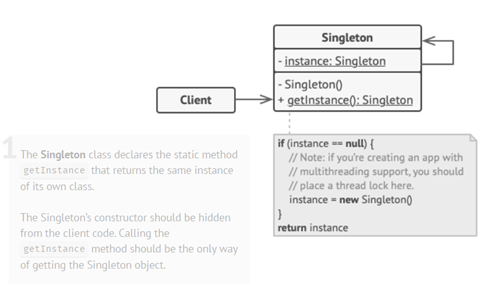
\includegraphics[width=1\textwidth]{../../img/schema_singleton.png}
    \caption{Schema del pattern Singleton}
    \label{fig:SingletonPattern}
    
\end{figure}

Il pattern Observer è utilizzato per notificare altri oggetti quando l'utente corrente cambia. La classe\texttt{CurrentOperator} definisce un'interfaccia \texttt{CurrentUserChangeListener}
che deve essere implementata da tutte le classi interessate ai cambiamenti dell'utente corrente.
\begin{figure}[H]
    \centering
    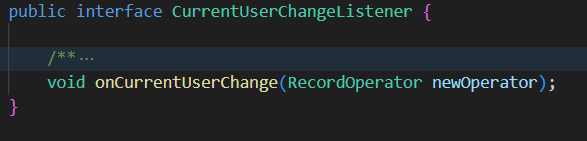
\includegraphics[width=1\textwidth]{../../img/currentUserChangeListener.png}
    \caption{Interfaccia CurrentUserChangeListener}
    \label{fig:Observer 1}
\end{figure}
La classe contiene metodi per aggiungere (\texttt{addCurrentUserChangeListener}) e rimuovere (\texttt{removeCurrentUserChangeListener}) listener interessati ai cambiamenti dell'utente corrente.
Quando l'utente corrente cambia, il metodo \texttt{notifyCurrentUserChange} viene chiamato per notificare tutti i listener registrati.
\begin{figure}[H]
    \centering
    \includegraphics[width=1\textwidth]{../../img/notifyCurrentUserChange.png}
    \caption{Metodo notifyCurrentUserChange}
    \label{fig:Observer 2}
\end{figure}
In questo modo, altre parti dell'applicazione possono essere avvisate quando l'utente corrente cambia, consentendo una gestione flessibile degli eventi correlati all'utente.

Questo pattern è stato implementato seguendo questo schema:
\begin{figure}[H]
    \centering
    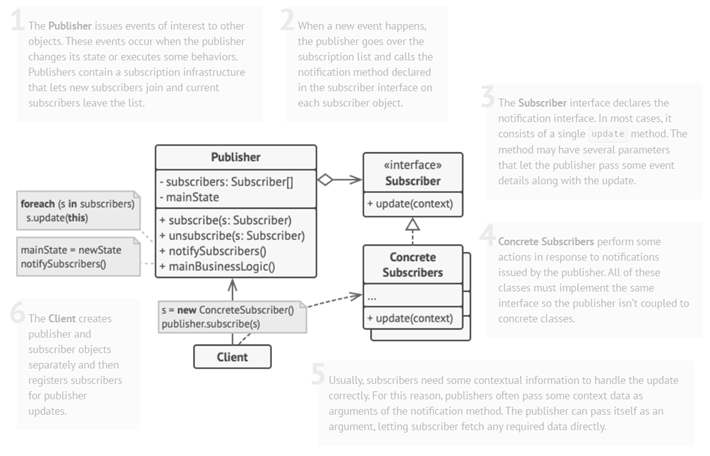
\includegraphics[width=1\textwidth]{../../img/schema_observer.png}
    \caption{Schema del pattern Observer}
    \label{fig:ObserverPattern}
\end{figure}

\end{document}